\documentclass{jsarticle}
\usepackage[dvipdfmx]{graphicx}
\usepackage{comment}
\usepackage{listings}
\usepackage{cases}
\usepackage{cprotect}
\lstset{
    basicstyle={\ttfamily},
    identifierstyle={\small},
    commentstyle={\smallitshape},
    keywordstyle={\small\bfseries},
    ndkeywordstyle={\small},
    stringstyle={\small\ttfamily},
    frame={tb},
    breaklines=true,
    columns=[l]{fullflexible},
    numbers=left,
    xrightmargin=0zw,
    xleftmargin=3zw,
    numberstyle={\scriptsize},
    stepnumber=1,
    numbersep=1zw,
    lineskip=-0.5ex,
    keepspaces=true,
    language=c
}
\renewcommand{\lstlistingname}{リスト}
\makeatletter
\newcommand{\figcaption}[1]{\def\@captype{figure}\caption{#1}}
\newcommand{\tblcaption}[1]{\def\@captype{table}\caption{#1}}
\makeatother

\title{プログラミング演習I 最終報告書}
\author{Ec4 32 平田蓮}
\date{}

\begin{document}
\maketitle

\section{プログラムの構成}
    今回プログラムを作成する上で基本的に授業資料\cite{text}を参考にした。
    しかし、コンピュータの思考プログラムを作成する際に、
    資料にある通りの二次元配列を利用したプログラムでは
    現代のPCでは限界のある計算量を要求してしまうため
    計算量を軽減できるビットボードを利用したゲームプログラムも実装した。
    コンピュータの思考プログラムは基本的にこちらのゲームシステムを利用して動く。

    各プログラムについての細かい説明は提出ファイルの\verb|readme.txt|を参照されたい。

\section{二次元配列プログラムとビットボードプログラムの比較}
    今回一番力を注いだ部分として、ビットボードプログラムの性能を記す。

    \subsection{空間計算量}
        二次元配列プログラムでは\verb|char|型の二次元配列で盤面情報を保持している。
        これに必要な空間計算量は、$8 \times 8$盤面で64バイトである。
        一方、ビットボードプログラムでは以下のような構造で盤面を保持している。

        \begin{numcases}
            {盤面}
            \verb|long long int black| \ (黒盤面) & \nonumber \\
            \verb|long long int white| \ (白盤面) & \nonumber \\
            \verb|long long int placeable| \ (着手可能マス) & \nonumber
        \end{numcases}

        これに必要な空間計算量は24バイトである。
        一見ビットボードプログラムの方が有用であるように思えるが、
        ビットボードを利用する欠点としては、
        整数値の各ビットをマスに見立てて使用するため
        c言語では64ビット整数である\verb|long long int|を利用した64マス盤面が最大となってしまう。
        一方二次元配列を利用すればPCのメモリが許す限りの大きさの盤面でプレイすることが可能である。
        そのため、今回作成したプログラムは二次元配列の方のみ$8 \times 8$以上でも任意の盤面サイズでプレイすることが可能である。

    \subsection{時間計算量}
        ビットボードプログラムは、ビット演算で様々な処理を行える特徴がある。
        そのため、時間計算量で大幅に二次元配列に対して利がある。
        
        例として$8 \times 8$盤面のコマの数を数えることを考える。
        二次元配列を利用したプログラムでは、
        愚直に全マスに対して駒があるかないかを調べれば良いのでかかる計算量は約64となる。

        一方ビットボードでは、各色の盤面に対してそのビットボードが何ビット立っているかを調べれば良い。
        これは、ビット論理積を使ってマスクをすることを利用すると約15の計算量で求めることができる。
        マスクとは、例えば二進数10111001と11110000のビット論理積を
        求めると10110000となり、ビット列の前半部分のみ取り出せるというような操作である。

        このように、ゲームを進める上でビットボードの方が計算が速く、
        素早く処理を行うことができる。
        今回作成したプログラムでは特に盤面の探索部分がとても計算量が大きいため、
        コンピュータによる最善手の探索時はビットボードを利用した。

        両者のプログラムにどの程度差があるかを調べるために、
        それぞれのプログラムで両手ランダム着手で1000試合を行なったときの
        実行時間を調べた。使用PCはMacBook Pro 2017である。

        結果として二次元配列プログラムは9.874秒、
        ビットボードプログラムは0.033秒であった。
        約300倍の差があることがわかる。

\section{工夫点}
    今回実装したプログラムのビットボード以外の工夫点をそれぞれ取り上げる。

    \subsection{盤面入力}
        オセロの入力を手で行うときはテキストにもあるように盤面上の座標を入力することが多いと考えられる。
        しかし、実際のオセロの盤面は数字での座標ではなく、
        列をアルファベット{\bf a〜h}で表し行を数字{\bf1〜8}で表すため、
        その様式にあった入力("c4"など)を行えるようにした。
        こうすることで、
        試合時などに盤面情報を他の人に伝えやすくなると考えられる。

    \subsection{盤面サイズの任意化}
        授業資料11ページにあるように、
        盤面のサイズを任意に設定できるようにした。
        (上でも述べたように、ビットボードプログラムでの上限は$8\times 8$である)

        初期盤面を保存しているcsvファイルの1行目は盤面サイズの情報である。
        これを読み込むことで二次元配列等のメモリ確保を行っている。
        また、後述する盤面保存の際も盤面のサイズを1行目に書き込むようにしている。

    \subsection{ひっくり返るコマの数の表示}
        マスにコマを置くときにいくつコマをひっくり返すことができるかは気になるものである。
        そこで、二次元配列プログラムではいちいち数えなくて
        良いように着手可能マスの表示を{\bf そこのマスにおいたときにひっくり返るコマ数}にした。
        これは着手可能マスを求める際に計算をして配列に値を保存することで実現している。

    \subsection{棋譜、盤面の保存、読み込み機能}
        オセロは棋譜を扱いやすいゲームとして有名である。
        コマに差異がなく、各手番でプレイヤーが決めることはコマを置く場所のみだからである。
        オセロの棋譜は単純にプレイヤーの置いた座標をつなげることで表される。
        例えば、次の盤面は\verb|d3c3c4e3d2e1f4g3e2d6|で表される。

        \begin{figure}[h]
            \centering
            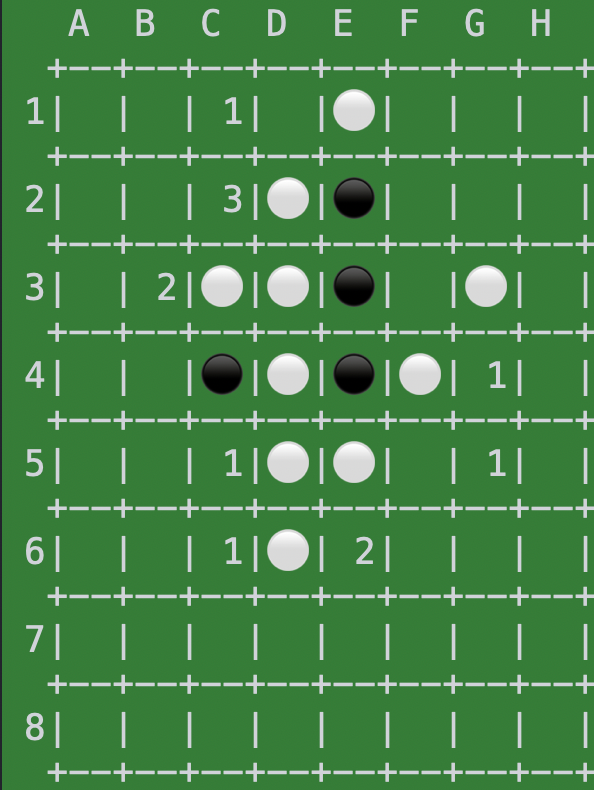
\includegraphics[width=6cm]{record_board.png}
            \cprotect\caption{\verb|d3c3c4e3d2e1f4g3e2d6|の盤面}
        \end{figure}

        今回作成した二次元配列プログラムでは、
        行われた試合の棋譜と盤面の保存機能と、
        棋譜を読み込んで盤面を展開する機能を実装した。
        実際には、寄付を読んだ際に先手後手をわかりやすくするために
        先手番はアルファベットの大文字、
        後手番は小文字を使って記録している。
        これにより、試合途中でも試合状況を保存して後から再開することができる。

    \subsection{やり直し機能}
        前節で述べた棋譜機能を使うと、着手のやり直しを行うことができる。
        具体的には、今の棋譜から後ろの2文字を取り除き、その棋譜で盤面を再現すればよい。
        この機能を搭載したことで、
        大会中などに操作ミスをした際に手間が減ると考えられる。

\section{コンピュータの思考アルゴリズム}
    コンピュータ対戦型のプログラムを作るにあたって、
    コンピュータの選手アルゴリズムを考える必要がある。
    過去に趣味でオセロAIを作ったことがあったが、
    その際はc言語以外の言語を利用したため、
    機械学習などが容易に行えたが、
    今回はc言語を使用するため大規模なプログラムは作成できないと判断し、
    単純な探索プログラムを作成した。

    使用した探索アルゴリズムはネガマックス法と呼ばれるもので、
    何手先まで読むかを決め、両プレイヤーが最善に打った場合
    どの手を打てば自分が一番有利になるかを探索するアルゴリズムである。

    \subsection{盤面評価値}
        探索をする上で大切になってくるのが盤面の評価値である。
        探索をした際に、最終的に有利、不利を評価する指標として数手先の盤面の評価値を用意する。
        実質的にこの評価値がオセロプログラムの強さを決めることとなる。

        今回は以下の三つの要素をもとに評価値を算出した。

        \begin{itemize}
            \item 石の数
            \item 石の配置
            \item 着手可能数
        \end{itemize}

        石の配置は、盤面の各マスに得点を設定し、
        そのマスに自分の石があれば得点を加算する方式で計算した。

        今回設定した得点は以下の通りである。(上下左右対象のため、一部のみ表示)

        \begin{figure}[h]
            \centering
            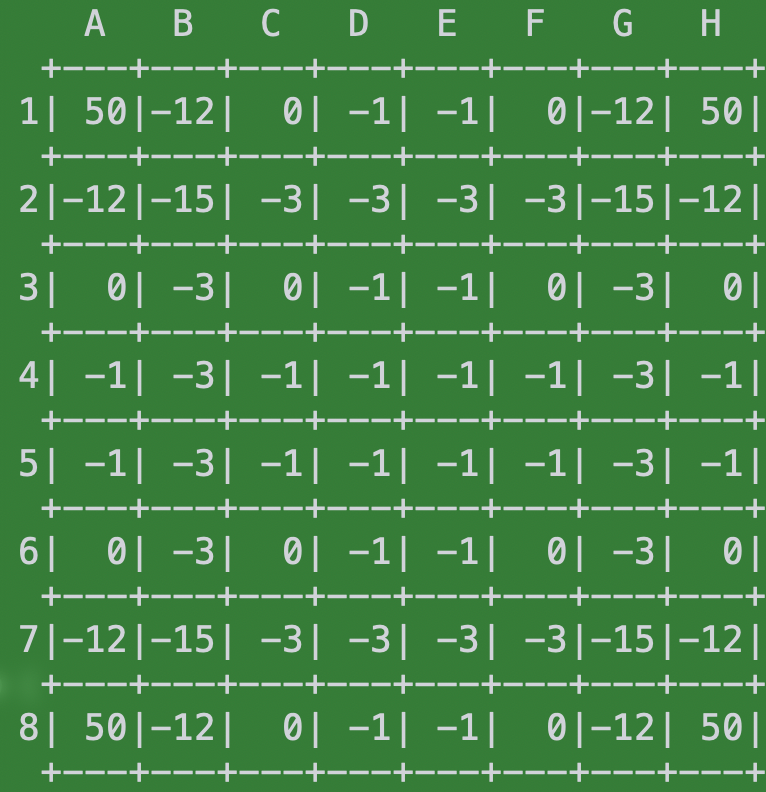
\includegraphics[width=8cm]{board_point.png}
            \cprotect\caption{各マスの得点}
        \end{figure}

        この他に確定石の数などの要素が考えられるが、
        あまりに複雑なプログラムを書かないといけないため、
        今回は実装しなかった。

        また、それぞれの要素の比率であるが、
        ゲームの進行度によって各要素の重要度が違うため、
        盤上のコマ数からゲームを4段階(序盤、中盤、終盤、最終盤)に分け、
        それぞれで比率を調節して評価値とした。

    \subsection{他のアルゴリズム}
        探索アルゴリズムの他にも、序盤の定石化や終盤完全読みなど、
        コンピュータのアルゴリズムとして使えるものは他にも考えられるが、
        今回は実装が困難と考え、探索アルゴリズムのみを使用した。
        機会があれば他のアルゴリズムも試したい。

\section{感想}
    今回の演習を経て、いくつか新しい知識を得ることができた。
    特にビットボードはそのうちの大きいものである。
    オセロだけでなく、囲碁や将棋などのゲームプログラムにも利用することができ、とても興味深いものだと思った。

    計算の速度が速くなるなど、ビットボードの利点は多く、
    授業では二次元配列だけでなくビットボードも扱うと
    プログラムの幅も広がり、面白いのではないかと思った。
    実際に、少し調べるとビットボードに関する様々な記事が出てくるだけでなく、
    理論的にもあまり難しくなく、
    自分で考えながら実装する楽しみも味わえた。

\begin{thebibliography}{99}
    \bibitem{text} "Ec4 プログラミング演習I"、上村健二、2020
    \bibitem{git} "BitboardReversi", https://github.com/tosik/BitboardReversi, tosik, GitHub, 2010
    \bibitem{nm} "ネガマックス法とネガスカウト法", http://www.nct9.ne.jp/m\_hiroi/light/pyalgo25.html, M.Hiroi, Algorithms with Python, 2007
\end{thebibliography}
\end{document}